To evaluate the results of KSVD, the learned dictionary atoms, as well as example signal reconstructions are examined. For the specific task at hand, it is known that piano music is sparse in the frequency domain, so the dictionary atoms should have learned meaningful frequency-domain content. To evaluate this, the \ac{FFT} of each atom was calculated. Figure \ref{fig:figs-atoms-png} shows the magnitudes of the \ac{FFT} for each atom sorted by the frequency of maximum component. From figure \ref{fig:figs-atoms-png}, it is clear that \ac{KSVD} has learned the primary frequencies of a variety of notes. It is important to note that the training data does not necessarily include every note on a piano, and this may be the reason that certain notes have multiple atoms while others do not have an atom. To evaluate the reconstructed data, several audio frames not seen in the training dataset are reconstructed using the learned dictionary and the \ac{OMP} algorithm. Figure \ref{fig:figs-reconstructed-png} shows a subset of one of these frames, approximated using 10 atoms, as well as all atoms from the dictionary.

\begin{figure}[h]
	\centering
	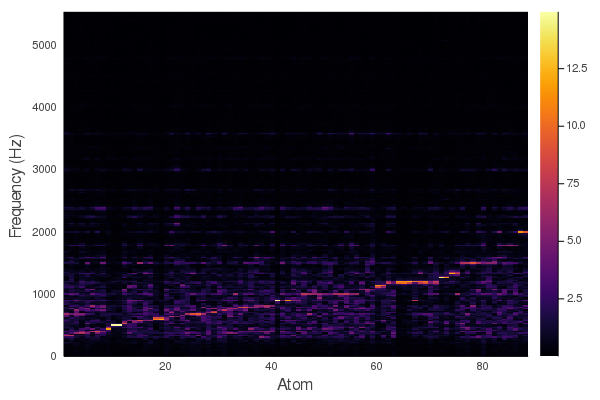
\includegraphics[width=0.5\textwidth]{figs/atoms.png}
	\caption{Learned Frequencies of Dictionary Atoms}
	\label{fig:figs-atoms-png}
\end{figure}

\begin{figure}[h]
	\centering
	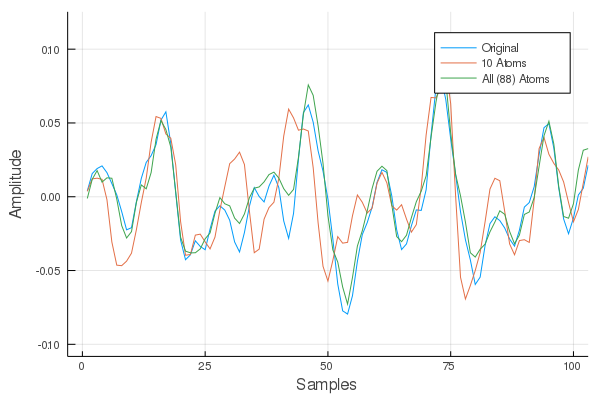
\includegraphics[width=0.45\textwidth]{figs/reconstructed.png}
	\caption{Example of Reconstructed Signal with 10 and 88 Atoms}
	\label{fig:figs-reconstructed-png}
\end{figure}
